\documentclass{beamer}
\usetheme{metropolis}  
\usecolortheme{wolverine}
\usepackage{hyperref}
\usepackage{bigints}
\title{Introducci\'on a la probabilidad y estad\'istica CM274}
 \usepackage[spanish]{babel}
\date{\today}
\author{C\'esar Lara Avila}
\institute{\url{https://github.com/C-Lara}}
\begin{document}
  \maketitle
  \section{1. Introducci\'on a la probabilidad }
  
 \begin{frame}{Introducci\'on a la teoria de conjuntos}
 \small{Un \underline{conjunto} es una colecci\'on desordenada de elementos.
 	
 Un conjunto $A$ con un n\'umero finito de elementos se denomina \underline{conjunto finito} y su tama\~no (n\'umero de elementos) se denota como $\vert A \vert$. Un conjunto con un n\'umero infinito de elementos se denomina \underline{conjunto infinito}.
 	
En muchos casos consideramos conjuntos indexados por un conjunto finito o infinito. Por ejemplo $U_a, a \in A$ representa m\'ultiples conjuntos, un conjunto para cada elemento de $A$. Para m\'ultiples conjuntos $U_a, a \in A$, definimos las operaciones de uni\'on e intersecci\'on, como sigue
 	
 	\begin{align*}
 	\bigcup_{a \in A} U_a &= \{u: u \in U_a \ \ \text{para uno  o m\'as} \ \ a \in A   \} \\
 	\bigcap_{a \in A} U_a &= \{u: u \in U_a \ \ \text{para todo} \ \ a \in A   \}. 
 	\end{align*}	
 }
 \end{frame}
 
 \begin{frame}{Introducci\'on a la teoria de conjuntos(1)}
\small{ \textbf{Ejemplo}
 Si $A_1 = \{1 \}, A_2 = \{1, 2 \}, A_3 = \{1, 2, 3\}$, tenemos:
 
 \begin{align*}
 \{A_i:i \in \{1,2,3\}\} &= \{\{1\}, \{ 1, 2\}, \{1, 2, 3 \}\}\\
 \bigcup_{i \in \{1, 2, 3\}} &= \{1, 2, 3 \} \\
 \bigcap_{i \in \{1, 2, 3\}} &= \{1 \}
 \end{align*}
 
 Los conjuntos $U_a, a \in A$ son \underline{mutualmente disjuntos} si $\bigcap_{a \in A} U_a  = \emptyset$ y son \underline {disjuntos dos a dos} si $a \neq b$ implica que $U_a \cap U_b = \emptyset$. La uni\'on de conjuntos disjuntos dos a dos $U_a, a \in A$ es denotado algunas veces como $\uplus_{a \in A}U_a$.	
 	}
 \end{frame}
 
  \begin{frame}{Introducci\'on a la teoria de conjuntos(2)}
 \small{El \underline{conjunto potencia} de un conjunto $A$, es el conjunto de todos los subconjuntos de $A$, incluyendo el conjunto vacio $\emptyset$ y $A$. Este conjunto es denotado por $2^ A$. Si $A$ es un conjunto finito entonces
 	
 	\[
 	\vert 2^A \vert = 2^{\vert A \vert}
 	\]
 	
 	El conjunto $U_a, a \in A$ forma una \underline{partici\'on} de $U$ si
 	
 	\[
 	\biguplus_{\alpha\in A} U_{\alpha} = U.
 	\]
 	
La generalizaci\'on  del tama\~no de un conjunto $A$ a conjuntos infinitos, puede hacerse notando que dos conjuntos finitos $A, B$ tienen el mismo tama\~no si y s\'olo si existe una biyecci\'on entre ellos, y generalizando esta noci\'on a conjuntos infinitos.
 	}	
\end{frame}
 

 \begin{frame}{Introducci\'on a la teoria de conjuntos(3)}
 \small{\textbf{Ley distributiva de conjuntos:}  Sean los conjuntos $U_a, a \in A$ y un conjunto $C$,
 \begin{align*}
 \Biggl( \bigcup_{a \in A} U_a  \bigcap C \Biggr) = \bigcup_{a \in A} \Biggl(U_a \bigcap C \Biggr)\\
 \Biggl( \bigcap_{a \in A} U_a  \bigcup C \Biggr) = \bigcap_{a \in A} \Biggl(U_a \bigcup C \Biggr)
 \end{align*}
 
 	
\textbf{(Ley de Morgan)} Sean los conjuntos $U_a, a \in A$,
  
\begin{align*}
\Biggl( \bigcup_{a \in A} U_a\Biggr)^c  = \bigcap_{a \in A}U_a^c \\
\Biggl( \bigcap_{a \in A} U_a\Biggr)^c  = \bigcup_{a \in A}U_a^c
 \end{align*}
  
   
}
 \end{frame}

 
  \begin{frame}{Definiciones b\'asicas }
  Probabilidad es el lenguaje para cuantificar la incertidumbre. 
  
 \textbf{\underline{Conceptos:}}
  \begin{itemize}
  	\item El \textbf{\underline{espacio muestral}} $\Omega$ de un experimento es el conjunto de todos los resultados o salidas del experimento.
  	\item  Puntos $\omega$ en $\Omega$ son llamados:
  	
  	 \textbf{\underline{elementos, realizaciones o resultados muestrales}}.
  	\item  Subconjuntos de $\Omega$ son llamados \textbf{\underline{eventos}}.
  \end{itemize}
   El espacio muestral de un experimento puede ser finito, infinito contable o infinito no contable. En particular el conjunto vacio $\emptyset$ y el espacio muestra $\Omega$ son eventos.
  \end{frame}
  
   \begin{frame}{Espacio muestral }
   	
   	Cuando el espacio muestral es finito, se puede visualizar como la figura siguiente. 
   	
   	\begin{figure}[h]
   		\centering
   		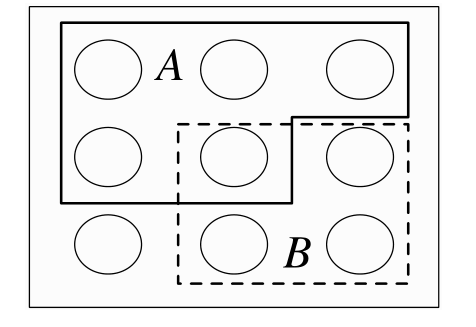
\includegraphics[width=6cm]{p1}
   	\end{figure}
   	\small{Cada \'ovalo representa una salida y un evento es un conjunto de \'ovalos $A$ o $B$.}
   	\end{frame}
 \begin{frame}{Casos de espacios muestrales}
 	
\begin{enumerate}
 \item \scriptsize {En el experimento aleatorio de lanzar una moneda tres veces y observar los resultados el espacio muestral es el conjunto $\Omega=\{CCC,CCS,CSC,CSS,SCC,SCS,SSC,SSS\}$. El evento $A=\{CCC,CCS,CSS,CSC\}\subset \Omega$ describe \texttt{una cara que se obtuvo en el lanzamiento de la primera moneda}. En este caso tanto el espacio muestral $\Omega$ como el evento $A$ son conjuntos finitos.}
 
 \item \scriptsize{ Considere un experimento aleatorio de lanzar un dardo en un tablero redondo, sin salirse del tablero. Suponiendo que el radio del tablero es $1$, el espacio muestral  es el conjunto de todos los vectores bidimensionales dentro del c\'irculo unitario $$\Omega=\left\{(x,y)\,:\, x,y\in\mathbb{R}, \,\sqrt{x^2+y^2} < 1\right\}$$. Un evento que describe un golpe en el tablero puede  puede ser,
 
 \[
 A=\left\{(x,y)\, : \,x,y\in\mathbb{R}, \,\sqrt{x^2+y^2} < 0.1\right\}\subset\Omega.
 \]
 
 En ambos casos el espacio muestral $\Omega$ y el evento $A$ son infinitos incontables.}
  \end{enumerate}
\end{frame}
\begin{frame}{Eventos  }
\begin{enumerate}
\item Para un evento $A$, el resultado del experimento aleatorio $ \omega \in \Omega $ est\'a en $A$ ($\omega \in A$) o   no est\' en  $A (w \notin A)$. En el primer caso, decimos que \underline{ el evento $A$ ocurri\'o}  y en el segundo caso decimos que \underline{el evento $A$ no ocurri\'o}.

\item $A \cup B$ es el \underline{evento de que $A$ o $B$ ocurren} y $A \cap B$ es el \underline{evento de que $A$ y $B$ ocurren}. El complemento $A^c$ ( el complemento en el conjunto universal se toma como $\Omega: A^c = \Omega -A$) representa \underline{el evento de que $A$ no ocurri\'o}. 

\item Si los eventos $A, B$ son disjuntos $(A \cap B = \emptyset)$, los \underline{dos eventos no pueden ocurrir al mismo tiempo}, ya que ning\'un resultado del experimento aleatorio pertenece tanto a $A$ como $B$. Si $A \subset B$ entonces si  $B$ ocurre implica que $A$ tambi\'en ocurre.
\end{enumerate}
\end{frame}

\begin{frame}{M\'as sobre eventos}
 Una lista de eventos se dice \underline{mutualmente exclusivo} si ning\'un elemento del espacio muestral pertenece a m\'as de un evento. Como lo muestra la siguiente figura:
 
 \vspace{0.2cm}
 
 \begin{figure}[!htb]
 	\centering
 	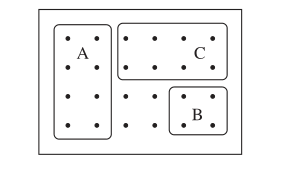
\includegraphics[width=6cm]{p3}
 \end{figure}
\scriptsize{Esto implica que  la ocurrencia de cualquiera de estos eventos  implica la no ocurrencia de los restantes  eventos}
\end{frame}

\begin{frame}{M\'as sobre eventos}
	
Cuando todos los elementos en un espacio muestral pueden ser encontrados en al menos un evento en una lista de eventos, entonces la lista de eventos se dice \underline{colectivamente exhaustivos}. 
	
	\vspace{0.2cm}
	
	\begin{figure}[!htb]
		\centering
		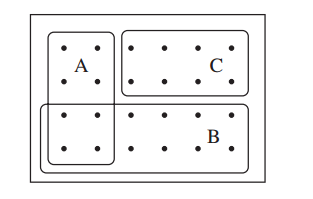
\includegraphics[width=6cm]{p4}
	\end{figure}
\scriptsize{En este caso ning\'un elemento del espacio muestral, es omitido y un \'unico elemento puede pertenecer a m\'as de un evento, como se muestra en la anterior figura:}
\end{frame}
\begin{frame}{M\'as sobre eventos}
Se dice que los eventos que son mutuamente exclusivos y colectivamente exhaustivos, forman una \underline{partici\'on del espacio muestral}. Como se muestra en la figura. 

\vspace{0.2cm}

\begin{figure}[!htb]
	\centering
	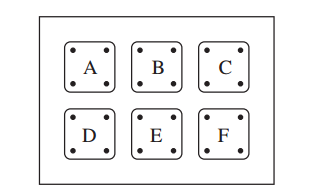
\includegraphics[width=6cm]{p5}
\end{figure}

Cualquier conjunto de eventos mutuamente excluyentes y colectivamente exhaustivos se denomina \underline{espacio de eventos}.

\end{frame}

\begin{frame}{Caso explicativo}
\begin{itemize}
\item \small{Secuencias de bits se transmiten a trav\'es de un canal de comunicaci\'on en grupos de cinco. Cada bit puede ser recibido correctamente o puede  ser modificado en tr\'ansito, lo que ocasiona un error. Consideremos un experimento que consiste en observar los valores de bits a medida que llegan e identificarlos con la letra $c$ si el bit es correcto y con la letra $e$ si el bit est\'a en error.} 

\vspace{0.2cm}

\scriptsize{El espacio muestral consta de $32$ resultados de $ccccc$ a $eeeee$, de cero bits transmitidos incorrectamente a los cinco bits que est\'an en error.
	
\vspace{0.2cm}
	
Sea el evento $A_i, i = 0,1, \dots, 5$, consistente de todos los resultados en los cuales los $i$ bits est\'an en error.  As\'i $A_0 = \{ccccc\}, A_1 = \{ecccc, ceccc, ccecc, cccec, cccce\}$ y as\'i sucesivamente hasta $A_5 = \{eeeee\}$. Los sucesos $A_i, i = 0, 1,\dots 5$, particionan el espacio muestral y por lo tanto constituyen un espacio de eventos.}



\end{itemize}
\end{frame}

\begin{frame}{Funci\'on  probabilidad}
Una funci\'on  probabilidad $\mathbb{P}$ es una funci\'on que asigna un n\'umero real a cada evento $A \subset \Omega$ y que satisface los siguientes tres axiomas:

\begin{enumerate}
	\item $\mathbb{P}(A) \geq 0$, \ \ \mbox{para todo evento}  \ $A$.
	\item $\mathbb{P}(\Omega) = 1$.
	\item Sean $A_n, n \in \mathbb{N}$ es una secuencia de eventos disjuntos  por pares $(A_i \cap A_j = \emptyset)$ siempre que $i \neq j$, entonces
	
	\[
	\mathbb{P}\Bigl(\bigcup\limits_{i= 1}^{\infty}A_i \Bigr) = \sum_{i = 1}^{\infty}\mathbb{P}(A_i).
	\]
\end{enumerate}
\end{frame}

\begin{frame}{Propiedades b\'asicas de la funci\'on  probabilidad}
Podemos derivar algunas propiedades de $\mathbb{P}$ desde los anteriores axiomas. 

\begin{enumerate}
	\item $\mathbb{P}(\emptyset ) = 0$.
	\item $A \subset B \rightarrow \mathbb{P}(A) \leq \mathbb{P}(B)$.
	\item $0 \leq \mathbb{P}(A) \leq 1$.
	\item $ \mathbb{P}(A^c) = 1-\mathbb{P}(A)$.
	\item $A \cap B = \emptyset \rightarrow  \mathbb{P}(A \cup B) = \mathbb{P}(A) + \mathbb{P}(B)$.
\end{enumerate}	


\end{frame}

\begin{frame}{Importantes propiedades de la funci\'on  probabilidad}

\begin{itemize}
\item \scriptsize{(Principio de inclusi\'on-exclusi\'on) Para dos eventos $A$ y $B$,
	
	\[
	\mathbb{P}(A\cup B) = \mathbb{P}(A) + \mathbb{P}(B) -\mathbb{P}(A \cap B)
	\]
	

En general el principio de inclusi\'on-exclusi\'on  se puede escribir como,

\vspace{0.2cm}

\begin{align*}
\mathbb{P}\Biggl(\bigcup_{i}^{n} A_i\Biggr) & = \sum_{i}\mathbb{P}(A_i) -\sum_{i < j}\mathbb{P}(A_i \cap A_j)\\
&  + \sum_{i < j < k}\mathbb{P}(A_i \cap A_j \cap A_k)\\
&  \vdots \\
& + (-1)^n\mathbb{P}(A_i \cap A_2 \dots A_n)
\end{align*}

El signo que precede a una suma con la intersecci\'on de $m$ conjuntos es $(-1)^{m + 1}$. La raz\'on para sumar sobre \'indices crecientes es evitar el doble conteo.

\vspace{0.2cm}

Se debe notar  que si los conjuntos son disjuntos dos a dos, las intersecciones anteriores son todas vac\'ias y por lo tanto tienen probabilidad cero y esto se reduce a la aditividad finita.}
\end{itemize}
\end{frame}

\begin{frame}{Importantes propiedades de la funci\'on  probabilidad}
	
	\begin{itemize}
\item \scriptsize{ ( Aditividad finita de la probabilidad) Para cada secuencia $A_1, \dots A_n$ de eventos disjuntos dos a dos (por pares) $(A_i \cap A_j) = \emptyset $ siempre que $i \neq j$), entonces,}


\[
\mathbb{P}(A_1 \cup \dots \cup A_n) = \mathbb{P}(A_1) + \cdots \mathbb{P}(A_n).
\]
\item \scriptsize{ Para una secuencia creciente o decreciente de eventos $\{E_n, n \geq 1 \}$, se cumple que}

\[
\lim_{n \rightarrow \infty}\mathbb{P}(E_n) = \mathbb{P}(\lim_{n \rightarrow \infty}E_n).
\]
\item \scriptsize{(Continuidad de la probabilidad) Si $A_n \rightarrow A $ entonces }

\[
\mathbb{P}(A_n) \rightarrow \mathbb{P}(A)  \qquad \mbox{si} \  n \rightarrow \infty
\]
\item \scriptsize{(Lema de Borel-Cantelli) Si se tiene  $\{ A_1, A_2, A_3, \dots \}$ una secuencia de eventos. La serie $\displaystyle \sum_{n =1}^{\infty}\mathbb{P}(A_n)$ converge, entonces} $\mathbb{P}\Biggl(\bigcap_{m =1}^{\infty}\bigcup_{n = m}^{\infty}\Biggr) = 0$.
\end{itemize}
\end{frame}


\begin{frame}{Ejemplo explicativo}
\small{Un profesor distraido escribi\'o  $n$ cartas y las sell\'o en sobres antes de escribir las direcciones en los sobres. Luego escribi\'o las $n$ direcciones en los sobres al azar. ?` Cu\'al es la probabilidad de que al menos una carta fue dirigida correctamente?.}

\vspace{0.2cm}
	
	
\scriptsize{El n\'umero total de formas en que uno puede escribir $n$ direcciones en $n$ sobres es $n!$. Por lo que el espacio muestral  contiene $n!$ puntos. Ahora calculamos el n\'umero de resultados en el cual  al menos un sobre se trata correctamente. 


\vspace{0.2cm}

Para hacer esto, sea $E_i$ el evento de que la $i$  \'esima carta es direccionada correctamente,  entonces $E_1 \cup E_2 \cup 
\cdots \cup E_n $ es el evento de que al menos una  carta es direccionada correctamente.

\vspace{0.2cm}

Para calcular $\mathbb{P}(E_1 \cup E_2 \cup \cdots \cup E_n)$, utilizamos el \underline{principio de inclusi\'on-exclusi\'on.}
}
\end{frame}

\begin{frame}{Ejemplo explicativo(1)}
	
\scriptsize{Desde que $\mathbb{P}(E_1 \cup E_2 \cup \cdots \cup E_n) $ hay $n$ t\'erminos de la forma $\mathbb{P}(E_i)$, $\binom{n}{2}$ t\'erminos de la forma $\mathbb{P}(E_i \cap E_j)$, $\binom{n}{3}$ t\'erminos de la forma $\mathbb{P}(E_i \cap E_j \cap E_k)$ y as\'i.
	
\begin{align*}
\mathbb{P}(E_1 \cup E_2 \cup \cdots \cup E_n) &= n\frac{(n -1)!}{n!} - \binom{n}{2}\frac{(n -2)!}{n!} + \cdots  + \\
&(-1)^{n -2}\binom{n}{n -1}\frac{[n - (n -1)]!}{n!} + (-1)^{n -1}\binom{n}{n}\frac{1}{n!}.
\end{align*}

\vspace{0.2cm}

Esta expresi\'on simplificada, es de la forma:

\[
\mathbb{P}(E_1 \cup E_2 \cup \cdots \cup E_n) = 1 - \frac{1}{2!} + \frac{1}{3!} - \frac{1}{4!}+ \cdots + \frac{(-1)^{n -1}}{n!}.
\]
}
\end{frame}
\begin{frame}{Funci\'on  probabilidad de un espacio muestral discreto}

\scriptsize{Para un espacio muestral finito (finito contable) $\Omega$ un evento conteniendo un \'unico elemento $A = \{\omega\}, \omega \in \Omega$ es llamado un \underline {evento elemental}. Para un espacio  muestral con $n$ elementos, supongamos que se nos da un conjunto de $n$ n\'umeros no negativos $\{ p_{\omega}: \omega \in \Omega\}$ que suman a uno, entonces existe  una funci\'on de probabilidad \'unica $\mathbb{P}$ sobre esos eventos tales que $\mathbb{P} (\{\omega\}) = p_{\omega}$.

Esta probabilidad se define para eventos arbitrarios a trav\'es de la propiedad de aditividad finita:

\[
\mathbb{P}(A)=\sum_{\omega\in A} \mathbb{P}(\{\omega\})=\sum_{\omega\in A} p_{\omega}.
\]

En la cl\'asica interpretaci\'on  de probabilidad sobre espacios  muestrales finitos, las probabilidades de todos los eventos elementales $\{ \omega\}, \omega \in \Omega$ son iguales. Desde que la funci\'on de probabilidad debe satisfacer $\mathbb{P}(\Omega) =  1$, tenemos $\mathbb{P}(\{\omega\})=\vert \Omega\vert^{-1}, \text{para todo}\quad \omega\in\Omega.$ Esto implica que bajo el modelo cl\'asico sobre un finito $\Omega$, tenemos

\[
\mathbb{P}(A)=\frac{\vert A\vert}{\vert \Omega\vert}.
\]

}
\end{frame}


\begin{frame}{Funci\'on  probabilidad de un espacio muestral continuo}
\small{Para un espacio muestral continuo de dimensi\'on $n$ (por ejemplo $\Omega = \mathbb{R}^n$), definimos la funci\'on de probabilidad cl\'asica como
 
 
 \[
 \mathbb{P}(A)=\frac{\text{vol}_n(A)}{\text{vol}_n(\Omega)},
 \]
 
 donde $\text{vol}_n(S)$ es el volumen n-dimensional del conjunto $S$. }
 
 \vspace{0.2cm}
 
 \scriptsize{El volumen 1-dimensional de un conjunto $S\subset \mathbb{R}$ es su \underline{longitud}. El volumen 2-dimensional de un conjunto $S\subset \mathbb{R}^2$ es su \underline{area}.  El volumen 3-dimensional de un conjunto $ S \subset \mathbb{R}^3$ es su \underline{volumen}. En general el volumen n-dimensional de $A$ es la n-\'esima integral de la funci\'on constante $1$ sobre el conjunto $A$.}
 
 
 \vspace{0.2cm}
 
 \scriptsize{\textcolor{blue}{Lectura:} Chapter 1 Probability Probability, Markov Chains, Queues and Simulation Willian J.Stewart Princeton University Press 2009.}
\end{frame}


\end{document}